\section{Spin Dependent EMC Effect}

Ever since its discovery~\cite{Aubert:1983xm,Bodek:1983ec}, it has been clear that the EMC 
effect~\cite{Geesaman:1995yd} embodies important new information about nuclear structure. Unfortunately, the information is so well encoded that there is as yet no consensus on what it is telling us. It has been argued forcefully (see for example Ref.~\cite{Thomas:2016bxx,Guichon:2018uew}) that the model independent fact that there is a very strongly attractive scalar mean field in nuclei leads to changes in the internal structure of bound nucleons that can not only explain the EMC effect but play a vital role in the binding of atomic nuclei~\cite{Stone:2017oqt,Stone:2016qmi}. 
%
    \begin{figure}[h!]
        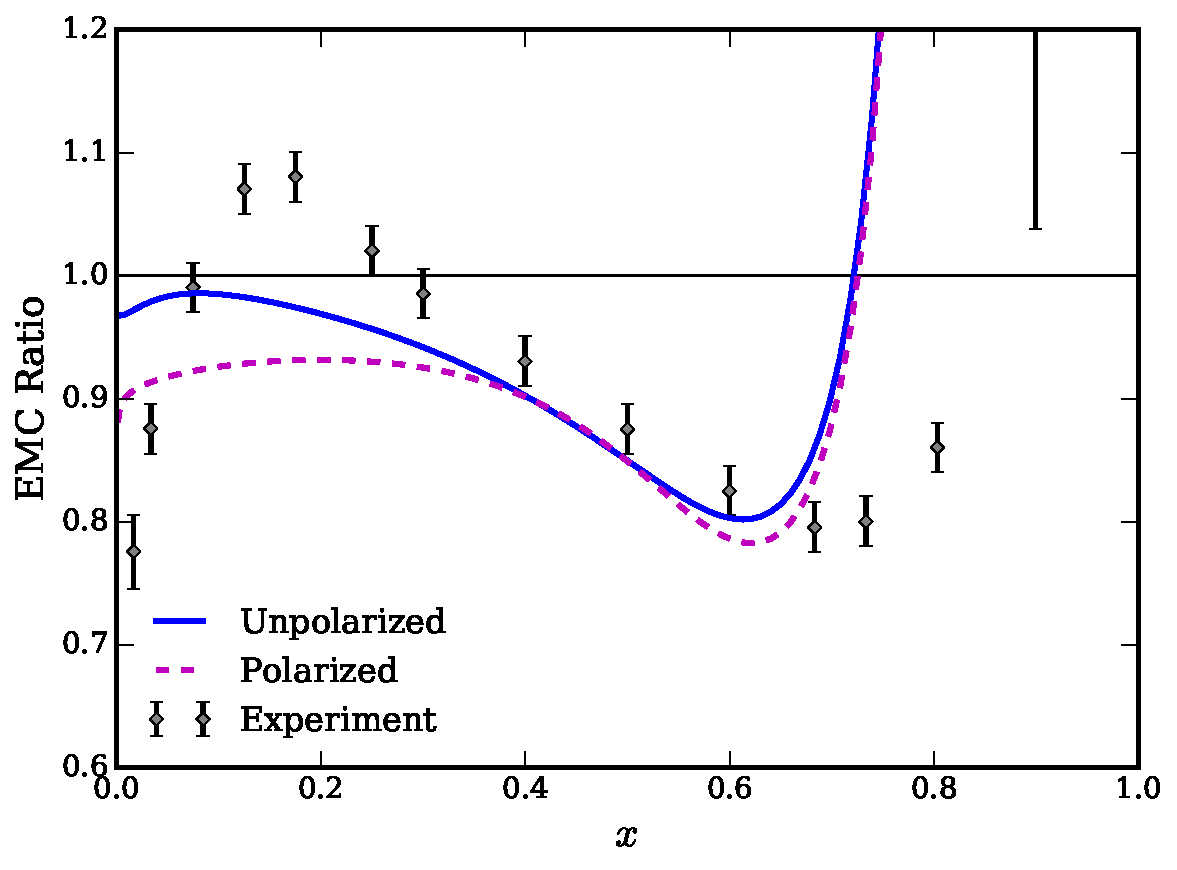
\includegraphics[width=0.5\textwidth]{plots/EMC_Com_NLO_PDF.pdf}
        \caption{Unpolarized and polarized EMC effect in the QMC model. The results are evolved to $Q^2=10$ GeV$^2$. The EMC data for nuclear matter is taken from Ref.~\cite{Sick:1992pw}.}
	\label{fig:EMC_Com}
    \end{figure}
%

In order to distinguish between the various proposals that have been made by way of explanation for the EMC effect it is vital to find new observables which may shed light on which is correct. Within a mean field approach, based upon the NJL model~\cite{Bentz:2001vc}, it was suggested that the isovector mean field in a nucleus with $N \neq Z$ would give rise to an isovector EMC effect~\cite{Cloet:2009qs,Bentz:2009yy}. In practice such an effect acts like an effective increase in the charge symmetry violation which is already present in nucleon PDFs 
because $m_d \neq m_u$~\cite{Londergan:2009kj} and leads to a substantial correction to the supposed NuTeV anomaly~\cite{Cloet:2009qs,Bentz:2009yy}.  A number of important proposals involving parity violating deep inelastic scattering have been made at Jefferson Lab which could clearly identify this novel aspect of the EMC 
effect~\cite{Cloet:2012td}.

Here we focus on the proposal of Clo\"et {\it et al.}~\cite{Cloet:2005rt,Cloet:2006bq} that it would be interesting to measure the modification of the polarized structure function of a bound proton. These investigators first studied the hypothetical case of the structure structure function, $g_1^p$, of a proton bound in nuclear matter.  The bound proton was assumed to be 100\% polarized and the effect of the medium was dramatic. The EMC effect was roughly twice as large for the spin dependent case as for the unpolarized case.  For comparison, if one were to take the extreme position that all of the EMC effect arises from high momentum (highly correlated) nucleons~\cite{Weinstein:2010rt}, it seems unlikely that there would be any effect on the spin structure function.

Strangely, even though the first calculation of the EMC effect within a self-consistent treatment of the modified structure of a bound nucleon was carried out 30 years ago~\cite{Thomas:1989vt}, there has so far 
been no calculation of the spin dependent EMC effect within that model -- the 
QMC model~\cite{Guichon:1995ue}. This is now of particular interest because it has been possible to derive an energy density functional equivalent to the QMC model, which starts with the modification of the quark structure of the nucleon in-medium, which has proven rather effective in nuclear structure studies~\cite{Guichon:2018uew,Stone:2017oqt,Stone:2016qmi}. 

A calculation of the polarized EMC effect was recently carried out within the QMC model by 
Tronchin {\it et al.}~\cite{Tronchin:2018mvu} and from the result shown in Fig.~\ref{fig:EMC_Com}, which is taken from that paper, we see that the prediction of the polarized EMC effect in the QMC model is about the same as that of the unpolarized effect.  We stress that this polarized EMC effect is defined for a proton which is 100\% polarized. In a real nucleus, such as $^7$Li, for which a measurement is planned at Jefferson Lab~\cite{JLab}, one needs to account for the fact that the polarization of the bound proton is less than that of the nucleus. 




